\section{Etat des lieux de l'éthique de l'\gls{ia}}

Cette section introduit les définitions qui seront utilisées dans ce rapport et qui sont indispensables à la compréhension du sujet. Comme en sociologie, les définitions sont un préalable pour une compréhension commune et éclairée et permettent la délimitation du périmètre des sujets. Au delà de l'aspect mathématique et statistique des algorithmes présentés dans ce rapport, il est tout aussi important de se questionner sur l'éthique des algorithmes et modèles déjà existants. \textit{A priori}, les termes utilisés seront, sauf exception, en français, bien que les équivalents anglophones soient davantage connus et usités. Le glossaire, en début de rapport, liste les équivalences.

\subsection{L'\gls{ia} : un, deux, trois, soleil ?}

\subsubsection{La génèse de l'\gls{ia}}
Aujourd'hui, l'\gls{ia} est un terme célèbre et hautement médiatisé, bien connu des citoyens sans toutefois avoir une idée claire de toutes les réalités que le terme désigne. Pourtant composé de deux termes \textit{a priori} anodins, l'\gls{ia} désigne tour à tour pour l'imaginaire collectif des robots, des machines, une réalité fantasmée ou crainte où ces entités sont soit au service de l'humanité ou soit source d'aliénation de cette dernière, à l'image des différents scénarios de films de science-fiction.


Née dans la première moitié du \siecle{20}, avec l'essor de la cybernétique, l'\gls{ia} désigne en premier lieu une discipline scientifique ayant pour finalité de créer des machines capables d'effectuer des tâches complexes, automatisées et guidées par des décisions éclairées en fonction des informations disponibles, à l'image de l'intelligence humaine.

Plus récemment, avec les progrès de l'informatique, de la collecte et du stockage des données, et des avancées scientifiques dans le domaine de la statistique, le grand public a uniquement connaissance des intelligences artificielles les plus médiatisées, comme AlphaGo et DeepBlue. Beaucoup d'\gls{ia} sont complètement inconnues, prenant des décisions mondialement importantes, telles qu'Aladdin de Blackrock pour la gestion automatisée d'actifs financiers à grande échelle, ou des décisions à haut risque telles que Kargu-2 l'\gls{ia} des drones autonomes tueurs. Le changement d'échelle entre le premier algorithme informatique et ces dernières \gls{ia} amène naturellement à se poser la question de l'éthique des algorithmes et des \gls{ia}, discutée dans la sous-section suivante \ref{subsection:ethique}.

Tout d'abord, le terme "intelligence" dérive du latin \textit{intelligencia}, référant à la compréhension et à la connaissance. L'intelligence réfère en général à l'intelligence humaine, i.e. cognitive, comme la capacité à formuler des pensées pour raisonner, anticiper ou s'adapter, faire, se souvenir ou créer.
Enfin, le terme "artificielle" est dérivé du latin \textit{artificialis}. Ce terme est composé du terme art du latin \textit{ars}, désignant l'ensemble des connaissances et des techniques pour atteindre un objectif, et du terme latin \textit{facio}, traduisant l'action de faire. À la fois le terme renvoie à la façon de faire dans l'état de l'art dans le sens premier et à la fois plus tardivement à la façon de contrefaire la nature.

En somme, l'\gls{ia} est l'ensemble des méthodes et des connaissances pour effectuer, à l'aide d'entités artificielles, des activités humaines simples ou complexes, impliquant une activité cognitive pouvant aller de la perception d'informations jusqu'à la prise de décision par un raisonnement éclairé. En ce sens, un algorithme prend en entrée des informations, procède à l'ensemble de ses instructions, souvent transposées d'activités cognitives humaines comme le raisonnement déterministe ou bayésien et rend compte d'un ou plusieurs résultats.

\subsubsection{Une définition opératoire arbitraire}
Afin de délimiter un premier périmètre, ce présent rapport donnera la définition suivante de l'\gls{ia} et se penchera sur l'entité opérationnelle plutôt que la discipline scientifique \footnote{Un ensemble de définitions est disponible en annexe \ref{appendice:definition-ia}} : une \gls{ia} est une entité informatisée ayant des fonctions relevant du traitement de l'information servant ou pouvant servir à la prise de décision. Tous les algorithmes informatisés sont inclus dans cette définition, y compris un simple "hello world". Dans ce dernier cas, l'\gls{ia} est rudimentaire car elle retourne presque surement l'information "hello world", ou n'importe quel même résultat de manière systèmatique, quelles que soient ses entrées. Même si l'information est de nature simple, la présence de ce résultat permet de déduire le bon fonctionnement de l'algorithme et du système ("healthcheck").

D'une part, la classe des algorithmes informatisés comprend l'ensemble des méthodes d'apprentissage statistique (ou \gls{ml} en anglais) dont les méthodes utilisant des réseaux de neurones profonds (ou \gls{dl} en anglais). Aujourd'hui, aux yeux du public, ces méthodes, en particulier le \gls{dl}, sont confondues avec l'\gls{ia} car leurs performances époustouflantes sont davantage sujettes à être exposées et promues par les médias et à les étiqueter comme l'\gls{ia} à part entière. D'autre part, les algorithmes d'\gls{ia}, dénommés \gls{gofai}, sont historiquement les premières créées et donc sans approche \gls{ml}, comme DeepBlue qui consistait uniquement à évaluer un grand nombre de positions avec une puissance de calcul importante.

De surcroît, les \gls{ia} sont qualifiées de faible si elles sont spécialisées uniquement dans une tâche ou possédant un nombre limité de fonctionnalités, alors que les \gls{ia} dites fortes seront capable de passer le test de Turing\footnote{Une \gls{ia} passe ce test si une personne n'est pas capable de différencier l'\gls{ia} d'un être humain, notamment au travers d'une conversation} et de surpasser l'intelligence humaine. À ce jour, aucune \gls{ia} n'a été qualifiée de forte.

\subsubsection{Un, deux, trois, soleil ?}


D'autres exemples d'IA :
* IA dans les voitures semi-autonomes
* 1.2.3 soleil
* système de recommandations
* matching
* westworld




\subsection{L'éthique : des graines à semer}\label{subsection:ethique}

Tout comme l'\gls{ia}, l'éthique est une notion qui recoupe plusieurs réalités. Par exemple, dans le sens commun, l'éthique renvoie souvent à l'éthique professionnelle comme le professionnalisme. L'éthique renvoie également à la justesse de la production d'un bien comme un café bio-éthique au sens équitable et respectueux de l'environnement.
L'éthique est d'abord une discipline philosophique de la morale et de la vertu. Le terme "éthique" dérive du latin \textit{ethicus} signifiant la morale, terme dérivé du grec \textit{êthikós} ayant la même signification. Pour comprendre pleinement la notion de l'éthique, il est nécessaire de comprendre la discipline philosophique en premier lieu. Dans la suite du rapport, les termes "morale" et "éthique" seront interchangeables, bien qu'aujourd'hui distingués par la philosophie moderne\footnote{Pour plus de détails, voir la vidéo du vidéaste Philoxime sur  \href{https://tournesol.app/entities/yt:HTAXqpMKm8M}{"L'éthique et la morale, quelle différence ?"}}.

\subsubsection{Un peu de philosophie : d'Aristote à Kant}

\paragraph{Aristote ou l'éthique des vertus}

La philosophie morale commence dès l'Antiquité avec les philosophes grecs : Socrate et ses disciples comme Platon, puis Aristote. La morale pour les philosophes socratiques désigne la conduite à tenir à travers les moeurs, dissertant entre ce qui est bien et ce qui est mal. Dans cette discipline, Aristote a produit quatre traités à propos de l'éthique : \citetitle{aristote-ethics-nico}, \citetitle{aristote-ethics-eud}, \citetitle{aristote-ethics-magna-moralia} et \citetitle{aristote-ethics-vertus-vices}. Dans ces traités, l'éthique pour Aristote, consiste à rechercher le bonheur (eudemonia) dans les vertus (arété) de la tempérance (sophrosúnê), de ne pas être dans l'excès, ni dans le manque, du courage et de la force d'âme (andreia), dans la justice, la légalité et l'intégrité (dikaiosunê), dans la prudence et la sagacité (phronêsis).

Concernant le droit de la cité et l'éthique, dans le livre V de l'\citetitle{aristote-ethics-nico} sur la justice, Aristote définit l'équité, une composante de l'éthique, comme une pratique à la discrétion du médiateur, pratique corrigeant les torts dues à une législation rigide et non applicable dans certains cas. L'éthique des vertus d'Aristote préfigurait déjà l'éthique comme précurseur du droit.

En somme, pour Aristote, la morale est avant tout composée de principes moraux à tenir au travers de sa conduite quotidienne de la vie, notamment le fait d'être juste et pour être juste, il faut pratiquer la justice au quotidien. Par conséquent, la philosophie morale disserte sur cette dernière, entendue aujourd'hui comme l'éthique, une discussion sur la morale.


\paragraph{Spinoza ou l'éthique de la connaisance, de la raison et des passions joyeuses}


Pour Spinoza, dans son ouvrage \citetitle{spinoza1894ethic}, la vertu, comme recherche des passions joyeuses et la mise à l'écart des passions tristes, est l'essence même de l'homme. L'homme libre est celui qui est capable de raison et d'user de ses connaissances sur les désirs et affects qui ont emprise sur ce dernier. Il s'agit alors de limiter l'emprise des passions tristes qui diminuent l'essence de l'être et de rechercher les passions joyeuses qui augmentent le conatus,\textit{i.e} la volonté et le désir d'exister\footnote{"
Plus chacun s'efforce et plus il est capable de chercher ce qui lui est utile, c'est-à-dire de conserver son être, plus il a de vertu ; au contraire, en tant qu'il néglige de conserver ce qui lui est utile, c'est-à-dire son être, il marque son impuissance.
"

"L'homme fort s'efforce donc, par cela même, autant qu'il est en lui, de bien agir et de vivre heureux." Scolie 73 livre IV

"l'effort pour se conserver soi-même est le premier et unique fondement de la vertu." Scolie 28 Livre IV}.



En somme, l'éthique spinozienne prône l'effort de la connaissance et de la raison et met en avant des valeurs morales positives comme la joie, l'amour, l'inclination et la béatitude. 


\paragraph{Bentham ou l'utilitarisme}


Bentham, dans son ouvrage \citetitle{bentham1771introduction}, définit le principe d'utilité comme étant toute action dont les conséquences augmentent ou diminuent le bonheur d'un agent\footnote{"By the principle of utility is meant that
principle which approves or disapproves of every action whatsoever.
according to the tendency it appears to have to augment or diminish the
happiness of the party whose interest is in question: or, what is the same
thing in other words to promote or to oppose that happiness"}. Ceci sera appelé ultérieurement utilitarisme hédoniste. Pour Bentham, le principe éthique est de maximiser l'utilité agrégée des agents. En effet, par la suite, dans la préface de \citetitle{bentham1776fragment}, Bentham étend le principe d'utilité au plus grand nombre\footnote{
"it is the greatest happiness of the greatest number that is the measure of right and wrong" (Preface of \citetitle{bentham1771introduction})}.

De manière plus générique, l'utilitarisme hédoniste est une philosophie morale conséquentialiste, qui met l'accent sur les conséquences de l'action.

\paragraph{Kant ou l'impératif catégorique}


En opposition au conséquentialisme, dans les \citetitle{kant1785fondements}, Kant introduit la notion d'impératif catégorique, qui est un principe que chaque agent rationnel s'impose avant toute action. L'impératif catégorique est un principe qui sous-tend l'action qui est accomplie par devoir en raison de ce principe. L'agent agit alors par devoir. L'éthique kantienne appartient à la famille des philosophies morales déontologiques, qui met l'accent sur les principes moraux et est qualifiée de déontologisme moniste.

En résumé, pour les trois premières philosophies morales présentées, l'éthique est avant tout la recherche de la vertu et du bonheur, l'eudémonisme. Pour Aristote, l'eudémonisme réside dans le juste milieu tandis que pour Spinoza, l'eudémonisme consiste en la connaissance, la raison et les passions joyeuses. Pour Bentham, l'eudémonisme recherché est global. \textit{A contrario}, pour Kant, l'éthique se situe avant tout dans les principes moraux qui justifient l'action.


Pour aller plus loin, ce rapport propose de mettre en perspective ces notions de manière séquentielle. Un agent possède des principes et des devoirs. Selon certaines situations, l'agent calcule en fonction de ses principes les résultats plausibles de son action. L'agent se prépare dans l'intention de faire l'action, puis l'exécute. L'action donne ou non des résultats et des conséquences. Le déontologisme moniste ou pluraliste se focalise sur les principes et les devoirs alors que le conséquentialisme se focalise sur les résultats et les conséquences de l'action.

\begin{figure}[ht]
  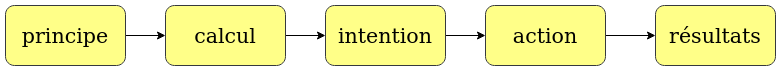
\includegraphics[width=\linewidth]{principeactionresultat.png}
  \caption{Modélisation séquentielle de l'action}
  % \vspace{-15pt}
\end{figure}
\subsubsection{De la philosophie morale vers des définitions pour l'ethique de l'\gls{ia}}

L'éthique, en philosophie morale avec ses diverses branches, revêt alors différents aspects, avec principalement une dichotomie entre l'éthique déontologique et l'éthique conséquentialiste. Se pose alors la question de savoir comment définir l'éthique de l'\gls{ia} ou plus globalement en sciences.

Concernant l'\gls{ia}, la définition de cette dernière donnée précédemment, implique l'utilisation de données en entrée, alimentant alors des programmes et des algorithmes, donnant lieu à des résultats et décisions en sortie. Sur chacune de ces composantes, il y a lieu de se poser la question si un caractère éthique peut s'y apposer ou non. Existe t-il des données éthiques et des données non éthiques ? Qu'est-ce qu'un algorithme éthique ? Une décision est t-elle toujours neutre ? Les résultats produits respectent-ils la confidentialité des données?

Pour répondre à la première question, il est nécessaire de se poser la question du protocole de collecte, de la représentativité, de l'absence de biais et de l'intégrité des données et des réponses. Cette question est cruciale pour les méthodes d'apprentissage statistique car les données constituent les fondements de l'apprentissage. Les predicteurs sont le fruit des données. En effet, les algorithmes apprennent à reproduire les biais non statistiques des données, tout en étant fortement sensibles aux biais statistiques.

Le choix d'un algorithme plutôt qu'un autre est aussi une question ouverte pour le statisticien, en marge de la performance. À l'instar des réseaux de neurones profonds, donnant des résultats spectaculaires mais difficilement explicables, le caractère boîte noire de certains algorithmes et non aisément auditable sont des obstacles à la compréhension de la reproduction éventuel de biais potentiellement dangereux.

De même, si les résultats obtenus et les décisions ont des conséquences dangereuses, faut-il les suivre indépendamment du fait qu'ils aient été obtenus à partir de données et d'algorithmes répondant ou non à un code déontologique ? Comment s'assurer de l'absence de biais dans les résultats ?

Pour les biais de représentativité, les algorithmes équitables\footnote{Il n'existe pas encore de traduction française officielle faisant consensus pour \gls{fairness}} (\gls{fairness} en anglais) peuvent répondre à cette problématique en ajoutant un terme de pénalisation quantifiant le degré du caractère inéquitable, à la manière des pénalisations statistiques classiques comme les régularisations dans les algorithmes de régression, et en s'assurant de la parité démographique\footnote{Soient S une variable aléatoire binaire sensible et $\hat{Y}$ le résultat du prédicteur construit avec les données, un algorithme répond à la contrainte de parité démographique si $P(\hat{Y}=1|S=0)=P(\hat{Y}=1|S=1)$} par exemple. 

Pour la confidentialité des données, les algorithmes à confidentialité différentielle (\gls{diffpriv} en anglais)\footnote{Un algorithme est dit $ (\epsilon,\delta)$-différentiellement confidentiel s'il répond R pour des données X et Y différent d'une entrée avec $P[R|X]<=e^\epsilon P[R|Y] + \delta$}  sont un compromis satisfaisant entre confidentialité des données privées et diffusion controlée de résultats.

Dans ce rapport, une \gls{ia} sera dite éthique si elle utilise des données éthiques à la fois pour les données d'apprentissage et les données réelles, des algorithmes auditables et produisant des résultats sécurisés sans biais. Compte tenu de cette définition forte, peu nombreuses sont les \gls{ia} répondant à cette définition, hormis les \gls{ia} trivialement simples.

De manière pratique, une \gls{ia} sera ici dite déontologique si elle a été conçue conformément à un code de déontologie. Cette définition permet d'inclure les \gls{ia} des organismes privés ou publics faisant un effort déontologique et d'encourager à produire des \gls{ia} encore plus éthique pour le bien commun.


\subsubsection{Vers une \gls{ia} plus éthique}

Aujourd'hui, bien que des comités et des réflexions éthiques émergent, la problématique de l'éthique en \gls{ia}, n'est pas suffisamment regardée avec l'importance nécessaire au regard de l'importance des impacts de l'\gls{ia} dans le quotidien des citoyens.
Notamment, les algorithmes de recommandation mis en place aujourd'hui visent à maximiser la rétention des utilisateurs sur les plateformes et poussent à consommer davantage, en exploitant les failles psychologiques de l'être humain déclenchant des mécanismes d'addiction. Dans ce domaine, les vidéos addictives et les sujets viraux exploitent des sentiments forts, comme la colère et la haine, et jouent sur le système de récompense à court terme lié à la dopamine. L'attention collective est alors saturée par des informations éventuellement moins importantes que d'autres plus cruciales à connaître pour le bien collectif, voire par des informations fausses.

Pour autant, un système de recommandation doit-il mettre en avant des contenus dits neutres ? Pour le cas des informations, la neutralité est une notion difficile à définir, car d'une part aussi factuelle que soit l'information, le parti pris de présenter l'information sous un angle plutôt qu'un autre est subjectif et d'autre part, il semble souhaitable de distinguer les informations vérifiables des informations fausses.
Concernant le monde des affaires, les entreprises en \gls{ia} possèdent des codes professionnels déontologiques avec ci-après une liste non exhaustive  : 

\begin{itemize}
    \item HuggingFace : \href{https://huggingface.co/blog/ethical-charter-multimodal}{Putting ethical principles at the core of the research lifecycle}
    \item IBM : \href{https://www.ibm.com/watson/assets/duo/pdf/everydayethics.pdf}{Everyday
Ethics
for Artificial
Intelligence}
    \item Fujitsu : \href{https://www.fujitsu.com/global/about/research/technology/aiethics/}{AI Ethics Impact
Assessment
From principles
to practice}
\end{itemize}

Les institutions et organismes publics formulent également des recommandations à toute échelle géographique, de national à international : 

\begin{itemize}
    \item Unesco : \href{https://unesdoc.unesco.org/ark:/48223/pf0000381137}{Recommendation on the Ethics of Artificial Intelligence
}
    \item UE : \href{https://futurium.ec.europa.eu/en/european-ai-alliance/blog/everyday-ethics-artificial-intelligence-guide-designers-and-developers}{Everyday Ethics for Artificial Intelligence: a guide for Designers and Developers}
    \item OCDE : \href{https://oecd.ai/en/ai-principles}{OECD AI Principles overview}
\end{itemize}

L'approche des différentes entreprises est plutôt déontologique que conséquentialiste, en listant diverses valeurs et principes moraux.


La première marche vers une \gls{ia} davantage éthique est la constitution d'une base de données éthique. Cela est justement le fondement premier de l'association Tournesol de constituer une base de données collaborative éthique pour servir à la fois de preuve de concept et de standard pour les analyses statistiques.